\chapter{Mobility Support}
\label{mobility support}

\section{Motivazioni per il supporto Mobile}

TCP / IP dispone di 3 livelli di protocollo superiori a quelli fisici:

\begin{figure}[H]
  \centering
  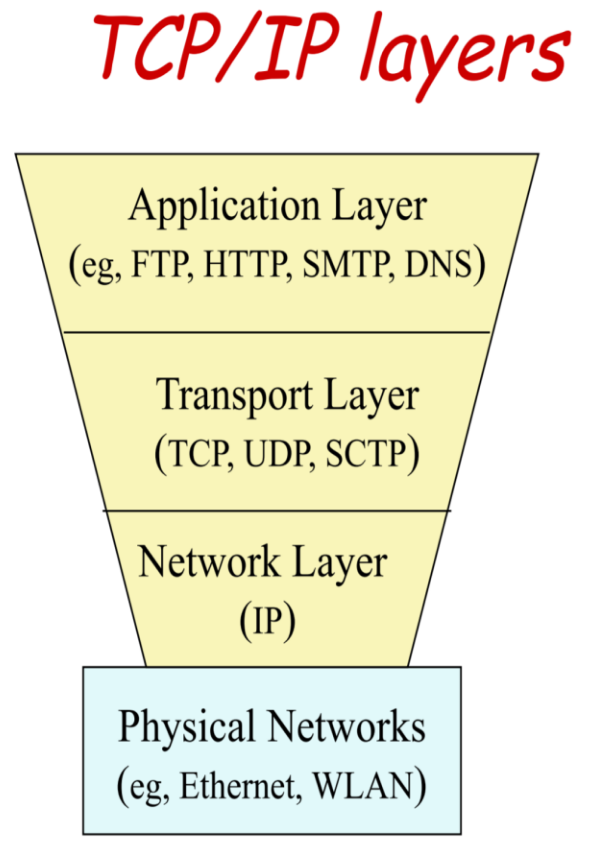
\includegraphics[scale=0.2]{tcp_ip_layers.png}
  \caption{TCP/IP layers}
  \label{fig:tcpiplayers}
\end{figure}

\textbf{Routing in Internet}

\begin{itemize}
  \item routing basato su prefissi: l'indirizzo IP di destinazione e il
prefisso di rete (es. 129.13.42) determinano la sottorete fisica
  \item un cambiamente della sottorete fisica implica un cambio
dell'indirizzo IP
  \item L'indirizzo IP è legato a una posizione (\textbf{point of attachment})
\end{itemize}

\textbf{Requisiti chiave per IP mobile}

\begin{itemize}
  \item \textbf{Raggiungibilità} - Un utente mobile deve rimanere
raggiungibile in qualsiasi momento attraverso un identificatore
permanente, indipendentemente dalla sua posizione attuale
(\textbf{subnet of attachment)}
  \item \textbf{Continuità} - Una comunicazione in corso non
dovrebbe interrompersi quando l'utente mobile si sposta (e va fuori dai
confini della sottorete)
\end{itemize}

\textbf{Requisiti desiderabili}

\begin{itemize}
  \item \textbf{Compatibilità} - Non dovrebbe esserci nessun cambiamento al
sistema corrente e ai routers
  \item \textbf{Trasparenza} - Continuità di comunicazione dopo l'interruzione
di un collegamento
  \item \textbf{Efficienza e scalabilità} - L'overhead dovrebbe essere
basso o nullo (in una tipica connessione a banda ridotta)
  \item \textbf{Sicurezza} - Autenticazione dei messaggi
\end{itemize}

\subsection{Problema e possibili soluzioni}

Nessuno degli strati TCP/IP è stato progettato per la mobilità.
I dispositivi mobili cambiano l'indirizzo IP mentre attraversano le
sottoreti e non sono più raggiungibili.

La modifica dell'indirizzo IP interrompe le connessioni del livello di
trasporto, quindi non c'è continuità. \\

\textbf{Tassonomia}

\begin{itemize}
  \item Scala: macro, micro
  \item Entità coinvolte nella gestione della mobilità: mobile-assistite,
network-only
  \item Mobilità di un nodo o di un gruppo
\end{itemize}

Come gestire la mobilità?\\

\textbf{Cambiare il livello IP / di rete} in modo tale che i livelli più alti
possano continuare a lavorare senza sapere nulla del cambiamento (soluzione
a livello di rete per la mobilità (es. MobileIP (v4, v6), GTP)

oppure...

\textbf{Cambiare il livello TCP / di trasporto} in modo tale che possa far
fronte ai cambiamenti degli identificatori degli end-point (soluzione a livello
di trasporto per la mobilità (es. Mobile TCP, SCTP)).

\textbf{Radice del problema}: l'indirizzo IP serve sia per la localizzazione,
sia come identificatore in connessioni TCP.

\subsection{Mobile IP}

\begin{figure}[H]
  \centering
  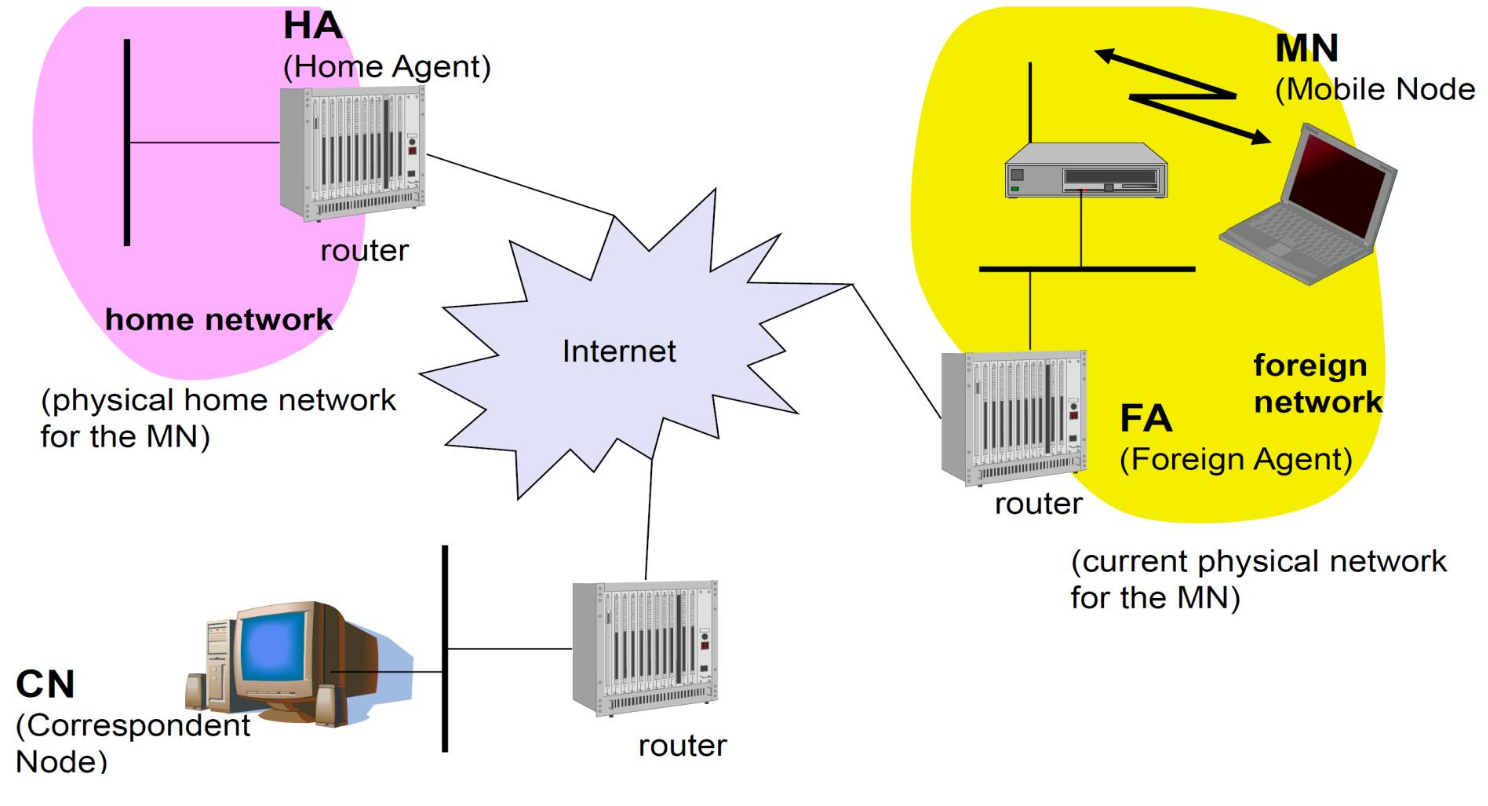
\includegraphics[scale=0.2]{mobileip1.png}
  \caption{Mobile IP, entità coinvolte}
  \label{fig:mobileip1}
\end{figure}

MN (Mobile Node) può spostarsi ed è in grado di rilevare un cambio di rete
rimanendo periodicamente in ascolto di segnali trasmessi dal FA (Foreign
Agent).

HA (Home Agent) mantiene il binding (home address, care of address,
duration of validity).

Care of address: IP temporaneo per un dispositivo mobile.

\begin{figure}[H]
  \centering
  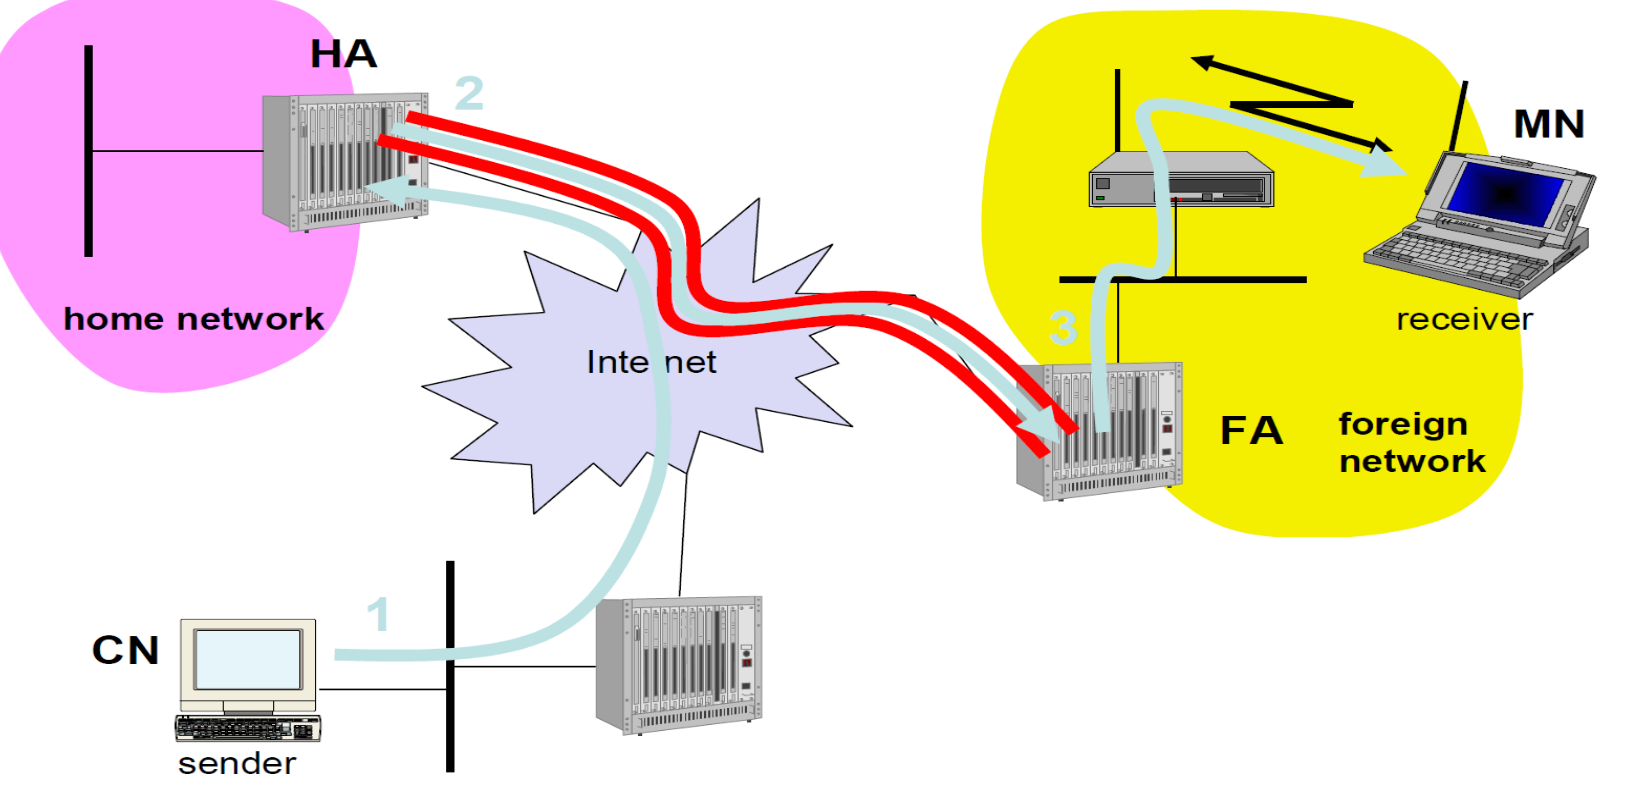
\includegraphics[scale=0.2]{mobileip2.png}
  \caption{Esempio mobile IP, CN -> MN}
  \label{fig:mobileip2}
\end{figure}

Quando i pacchetti arrivano all'home address, l'Home Agent HA apre un tunnel
IP-in-IP (in rosso nell'immagine) verso il foreign agent FA e manda i 
pacchetti, che li manda a sua volta al nodo mobile, al suo nuovo indirizzo.

Il tunneling IP-in-IP significa che il pacchetto IP originale è incapsulato
in un altro pacchetto IP con il nuovo indirizzo di destinazione (nuovo care
of address).

\begin{figure}[H]
  \centering
  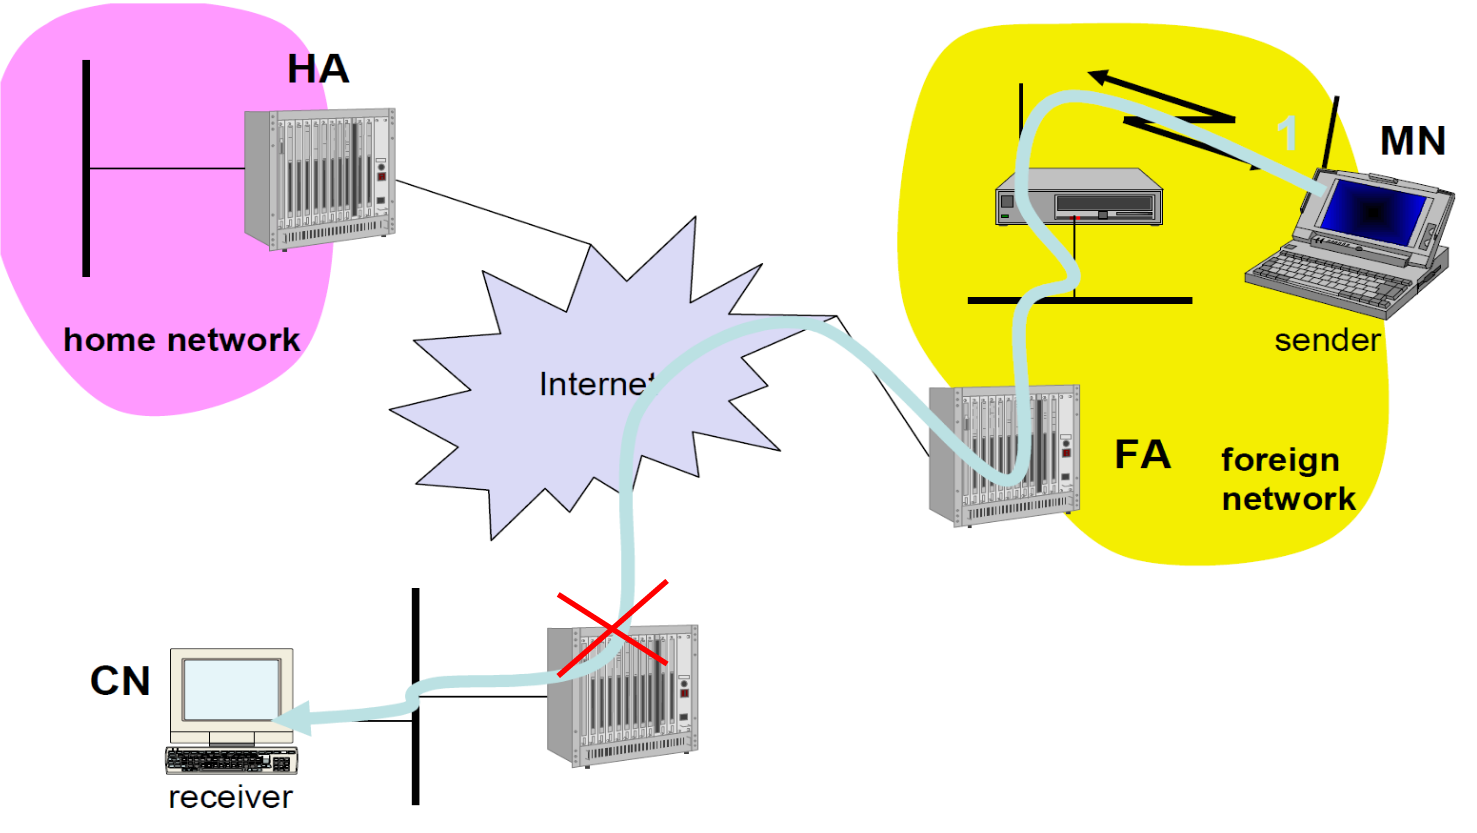
\includegraphics[scale=0.2]{mobileip3.png}
  \caption{Esempio mobile IP, MN -> CN}
  \label{fig:mobileip3}
\end{figure}

Il nodo mobile può inviare una risposta direttamente o con un
reverse tunnel (es. firewall scenario) attraverso l'home agent HA
(l'home agent rigira la risposta al destinatario). \\

\textbf{Mobile IP - Aspetti negativi}

\begin{itemize}
  \item \textbf{Sicurezza} - Un codice malevolo può
dichiarare un nuovo care-of-address e rubare i pacchetti in arrivo
al nodo mobile.
Per evitare questo, l'home agent HA e il nodo mobile devono condividere
una chiave segreta e autenticare le loro comunicazioni
  \item \textbf{routes più lunghe} - I pacchetti devono percorrere una
distanza extra fino all'home agent HA e poi indietro (triangle routing).
MN potrebbe inviare direttamente il care-of-address al CN
che lo usa successivamente -> problemi di sicurezza / privacy!
  \item \textbf{Filtro dei pacchetti}
ISPs possono bloccare i pacchetti in arrivo da un nodo mobile se l'indirizzo
d'origine è il vecchio home address e non appartiene al blocco di IP della
rete corrente.
\end{itemize}

\textbf{Mobile IP - Aspetti positivi}

\begin{itemize}
  \item Risolve il problema della mobilità alla radice (IP è il livello più
basso di TCP/IP)
  \item Tracking-support integrato (con un indirizzo IP permanente e home agent
HA)
  \item Nessun cambiamento al core della rete (solo i routers di confine,
gli HA sono coinvolti) 
  \item Privacy della località
\end{itemize}

\textbf{Mobile IPv6}

\begin{itemize}
  \item In IPv6, la funzionalità del foreign agent FA è integrata nel nodo
mobile stesso
  \item L'ottimizzazione delle routes è una parte integrante del protocollo
  \item Sicurezza integrata
\end{itemize}

\section{Sistemi mobili cellulari}

\subsection{Disambiguazione}

\begin{enumerate}
  \item E-UTRA(N) - Evolved UMTS Terrestrial Radio Access (Network)
  \item Super 3G - Riferito a LTE
  \item 3.9G - Usato per indicare che LTE non è il 4G
\end{enumerate}

\textbf{Set di requisiti richiesti da ITU-R (Radiocommunication Sector)
dell'ITU (International Telecommunication Union) nel 2008 per il 4G:}

\begin{itemize}
  \item Basato su protocolo IP
  \item Interoperabilità con tutti gli standard wireless esistenti
  \item Un data rate nominale di 100 Mbit/s (su mobile) e 1 Gbit/s (quando
client e stazione sono in posizioni fisse (relative))
  \item Condivisione e utilizzo dinamico delle risorse della rete per
supportare più utenti per cella.
  \item Banda dei canali scalabile 5–20 MHz, fino a 40 MHz
  \item Efficienza massima di 15 bit/s/Hz in downlink, e 6.75
bit/s/Hz in uplink
  \item Connettività senza interruzioni e roaming globale attraverso reti
diverse, con handovers/handoff leggeri
  \item Efficienza per il sistema: 3 bit/s/Hz/cell in downlink
e 2.25 bit/s/Hz/cell per uso domestico
  \item Capacità di offrire un'alta qualità del servizio per il supporto
multimediale
\end{itemize}

\begin{figure}[H]
  \centering
  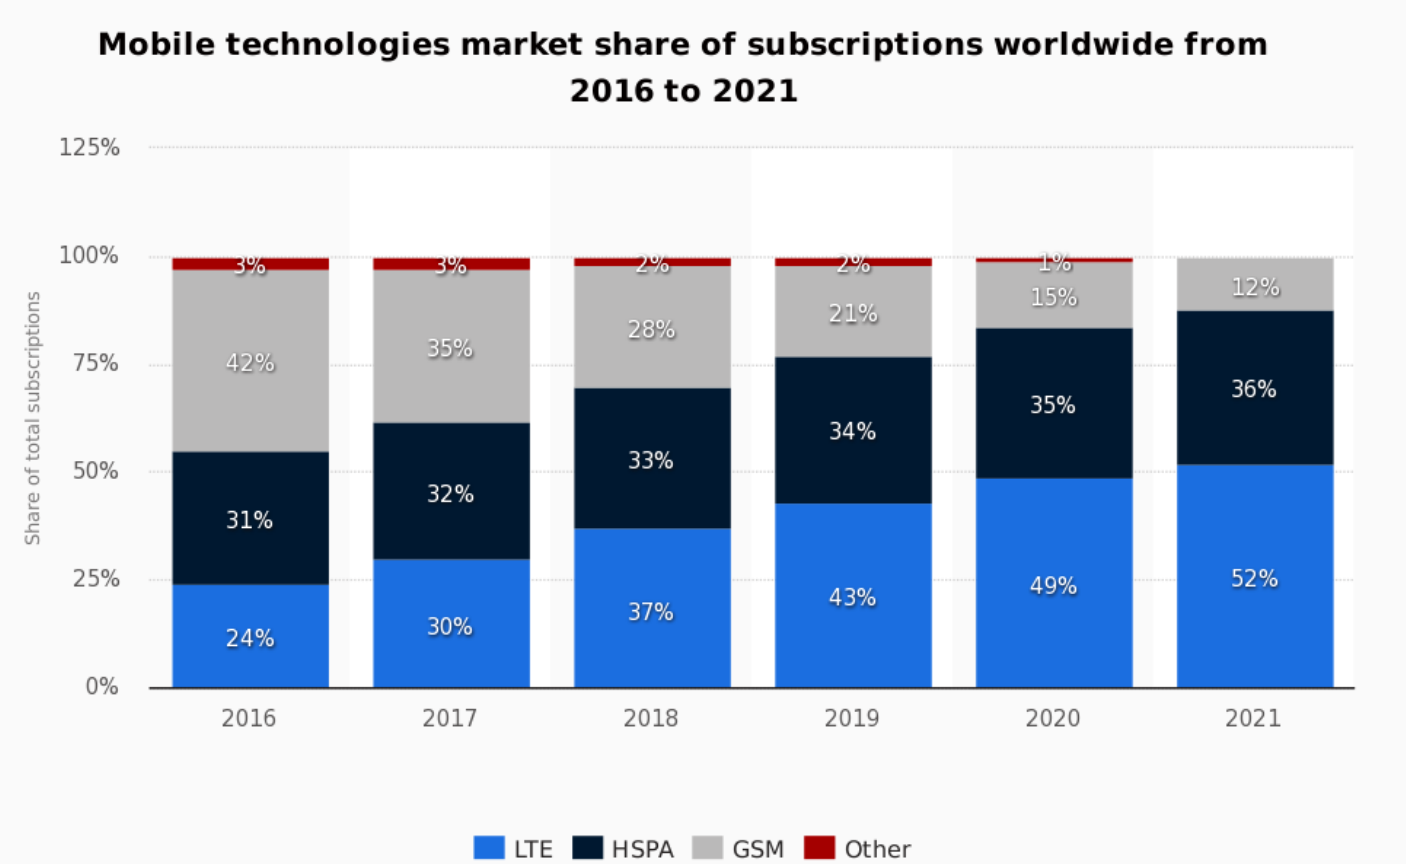
\includegraphics[scale=0.3]{mobtech.png}
  \caption{Previsione delle quote di mercato degli abbonamenti alle tecnologie
mobili in tutto il mondo dal 2016 al 2021}
  \label{fig:mobtech}
\end{figure}

\subsection{GSM}

GSM (Sistema globale per le comunicazioni mobili) è uno standard
sviluppato da ETSI (European Telecommunications Standards Institute) con lo
scopo di descrivere i \textbf{protocolli per la seconda generazione 2G} di reti
cellulari digitali per utenti mobili. \\

A partire dal 2014, è diventato lo standard mondiale de-facto per le
comunicazioni mobili con oltre 90 \% di mercato, operante in oltre 219 paesi
e territori.

Le reti 2G sono state sviluppate per sostituire le reti analogiche cellulari
di prima generazione (1G).

Lo standard GSM si è ampliato nel tempo fino a includere comunicazioni di
dati, dapprima grazie a un trasporto circuit-switched, poi tramite GPRS
(General Packet Radio Services) e EDGE (Enhanced Data rates for GSM
Evolution, or EGPRS)

Successivamente, il 3GPP ha sviluppato gli standard UMTS di terza generazione
(3G), seguiti da quelli di quarta generazione (4G) LTE standard avanzati,
che non fanno parte degli standard ETSI GSM.

\subsubsection{Storia...}

\textbf{1982 - nasce il gruppo speciale per la mobilità}

\textbf{1989} - European Telecommunications Standardization Institute
(ETSI) si assume la responsabilità di creare degli standard e cambia nome:
Global System for Mobile (GSM) communication

\textbf{1990} - Primo lancio ufficiale commerciale in Europa

GSM è la più popolare tecnologia 2G. La figura \ref{fig:gsm_table} mostra
alcune delle sue caratteristiche principali:

\begin{figure}[H]
  \centering
  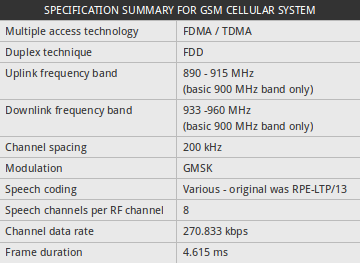
\includegraphics[scale=0.7]{gsm_table.png}
  \caption{Tabella riassuntiva delle specifiche dello standard GSM Cellular
System}
  \label{fig:gsm_table}
\end{figure}

Una delle caratteristiche fondamentali di GSM è il \textbf{Subscriber Identity
Module}, comunemente conosciuto come una carta SIM.

La SIM è una smart card rimovibile contenente l'abbonamento dell'utente, le
sue informazioni e la sua rubrica telefonica.

Questo consente all'utente di mantenere i propri dati cambiando dispositivo.

In alternativa, l'utente può anche cambiare operatore mantenendo il
proprio dispositivo, semplicemente cambiando la SIM.

Alcuni operatori possono bloccare questa possibilità, permettendo a un
telefono di utilizzare una sola SIM, o solo una SIM emessa da quell'operatore;
questa pratica è conosciuta come blocco SIM.

\subsubsection{GSM – Architettura funzionale}

Una \textbf{rete GSM} comprende molte unità funzionali.
Può essere suddivisa in:

\begin{itemize}
  \item \textbf{Base station subsystem} (BSS) - stazione di base
  \item \textbf{Network and Switching Subsystem} (NSS) - la parte della
rete più simile a una rete fissa, a volte chiamata core network.
  \item \textbf{GPRS Core Network} (GPRS) - la parte \textbf{opzionale} che
permette connessioni Internet basate su pacchetti (vedi sezione \ref{sec:gprs})
  \item \textbf{Operations support system} (OSS) - manutenzione della rete
\end{itemize}

I componenti aggiuntivi dell'architettura GSM comprendono database e
\textbf{funzioni di messaggistica}:

\begin{itemize}
  \item VLR : Visitor Location Register
  \item HLR : Home Location Register
  \item AUC : Authentication Center
  \item BTS : Base Transceiver Station
  \item OMC : Operation Maintenance Center
  \item EIR : Equipment Identity Register
\end{itemize}

\begin{figure}[H]
  \centering
  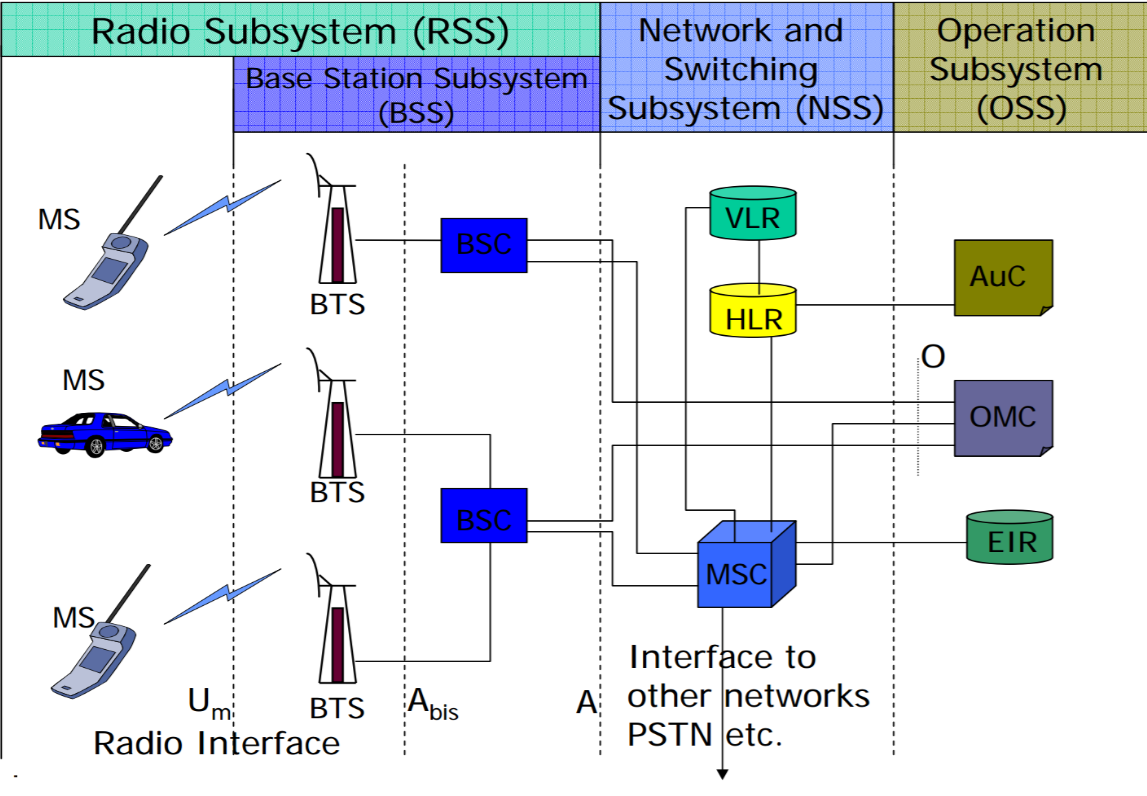
\includegraphics[scale=0.3]{archGSM.png}
  \caption{Struttura di una rete GSM}
  \label{fig:archGSM}
\end{figure}

Le stazioni di base (BTS) sono organizzate in piccoli gruppi, controllate da
una stazione di base di controllo (BSC) che è tipicamente co-localizzata in una
delle stazioni di base.

Tutto il sistema, composto dal BSC con i suoi BTS associati si chiama
\textbf{sottosistema di stazioni di base} (BSS). \\

Addentrandosi nella reta, c'è la zona principale di commutazione, nota come
\textbf{switching center mobile} (MSC).

Associati ad essa, ci sono i \textbf{registri di posizione}, cioè gli
home location registers (HLR) e i visitor location register (VLR) che tengono
traccia della località degli utenti mobili e consentono alle chiamate di
essere instradate a loro\\

Inoltre, ci sono il centro di autenticazione (AuC) e il equipment identify
register (EIR), utilizzati per l'autenticazione dei messaggi prima
che siano immessi sulla rete e per la fatturazione.

La MS e la BSS comunicano attraverso l'interfaccia Um (nota come
air-interface)

Il BSS comunica con il centro di Network Service Switching (NSS) attraverso
l'interfaccia A.

GSM è una rete cellulare, il che significa che i telefoni si
connettono ad essa tramite la ricerca di celle nelle immediate vicinanze.
Ci sono cinque tipi di celle, in base alle dimensioni, in una rete GSM:
celle \textit{macro, micro, pico, femto e umbrella}.

\section{General Packet Radio Service}
\label{sec:gprs}

General Packet Radio Service (\textbf{GPRS}) è un servizio per mobile orientato 
a pacchetti sui sistemi GSM in 2G e 3G. Viene attualmente mantenuto dal 3rd 
Generation Partnership Project (3GPP).

L'utilizzo della rete GPRS viene addebitato in base al volume dei dati 
trasferiti.

GPRS è un servizio di tipo \textit{best-effor}, che implica throughput e 
latenza variabili che dipendono sul numero di utenti che condividono il
servizio in modo concorrente, in opposizione allo switching dei circuiti,
dove una certa qualità dei servizi (QoS) è garantita durante la connessione.

Nei sistemi 2G, GPRS fornisce un data rate di 56-114 kbit/s.\\

La tecnologia 2G combinata con il GPRS viene a volte descritta come 2.5G,
che è una tecnologia tra la seconda (2G) e la terza (3G) generazione di 
telefonia mobile. Il 2.5 è un tentativo di migliorare i servizi sui dati 
del 2G.

Collega le reti GSM alle reti IP (è praticamente uno strato aggiunto dei 
servizi sui dati nella rete 2G). Data rate massimo: 57-171 bit/s.

\subsubsection{GPRS - Quality of Service}
\begin{itemize}
  \item Precedenza del servizio (high, normal and low priority groups)
  \item Affidabilità
  \item Ritardo
  \item Throughput
\end{itemize}

\subsubsection{LTE – Definitions}

\begin{itemize}
  \item EPC (Evolved Packet Core): la nuova architettura core dei pacchetti 
  definita in 3GPP Rel-8
  \item SAE (System Architecture Evolution): l'elemento della 3GPP per
definire le specifiche EPC
  \item LTE (Long Term Evolution): l'elemento 3GPP che ha sviluppato la tecnologia
  per l'accesso radio e E-UTRAN
  \item EPS (Evolved Packet System): termine 3GPP che si riferisce ad un sistema 
  end-to-end completo, che è UE, E-UTRAN e Core Network (EPC)
  \item E-UTRAN - la RAN (radio access network) che implementa l'interfaccia per la 
  tecnologia radio LTE
\end{itemize}

\subsection{UMTS - Universal Mobile Telecommunications System}

Il Universal Mobile Telecommunications System (\textbf{UMTS}) è un sistema 
mobile cellulare di terza generazione per reti basate sullo standard GSM.

Sviluppato e mantenuto dal 3GPP, UMTS è un componente del International
Telecommunications Union IMT - 2000 standard set.

UMTS usa la tecnologia per l'accesso radio wideband code division multiple 
access (W-CDMA) per offrire un'efficienza spettrale e larghezza di banda maggiore
per gli operatori mobile.

UMTS specifica un sistema di rete completo, che include l'accesso a reti radio
(UMTS Terrestrial Radio Access Network, or UTRAN), la core network 
(Mobile Application Part, or MAP) e l'autenticazione degli utenti attraverso 
le schede SIM (Subscriver Identity Module).

La tecnologia descritta in UTMS viene spesso riferita come 3GSM.

\subsection{User equipment}

Nell'UMTS e 3GPP LTE, lo user qeuipment (UE) è un qualsiasi dispositivo utilizzato 
da un utente finale per comunicare.

Può essere gestito da un telefono, un laptot con un adattatore mobile broadband, 
o qualsiasi altro device. \\

User Equipment (UE) comprende:

\begin{itemize}
  \item Mobile Termination (MT) module (gestisce tutte le funzioni per la
  comunicazione)
  \item Terminal Equipment (TE) module (termina lo stream dei dati)
  \item Universal Integrated Circuit Card (UICC) module (conosciuto come SIM card
per l'equipment LTE. Esegue un'applicazione chiamata Universal Subscriber
Identity Module (USIM))
\end{itemize}

\subsection{UTRAN - UMTS Terrestrial Radio Access Network}

Primarily a part of the 3G Mobile Communication Technology and defined as a
collective term for the BTS and Radio Network Controllers which make up the
UMTS radio access network.

Può trasportare molti tipi di traffico, dal real-time Circuit Switched all'IP 
based Packet Switched.

UTRAN permette la connettività tra l'user equipment e la core network.

UTRAN contiene le stazioni base, che sono chiamate Node Bs, e i Radio
Network Controllers (RNC).
RNC fornisce le funzionalità di controllo per uno o più Node Bs.
Un Node B e un RNC possono essere lo stesso dispositivo.

\subsection{E-UTRAN - Evolved Terrestrial Radio Access Network}

E-UTRAN è l'architettura di rete definita per l'interfaccia radio E-UTRA 
come parte della specifica per il layer fisico 3GPP LTE.

Gestisce le comunicazioni radio tra mobile e l'Evolved Packet Core.

Un unico componente: la stazione base evoluta, chiamata \textbf{eNodeB} o eNB.

\begin{figure}[H]
  \centering
  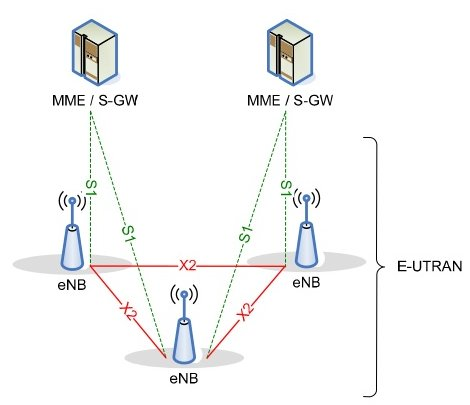
\includegraphics[scale=0.6]{utran_net.jpg}
  \caption{Architettura E-UTRAN}
  \label{fig:utran_net}
\end{figure}

L'eBN invia e riceve trasmissioni radio a tutti i dispositivi mobile che usano la 
stessa funziona di processing dei segnali analogici e digitali dell'interfaccia aerea LTE.

eNB controlla le operazioni di basso livello di tutti i suoi dispositivi inviando loro
messaggi di segnalazione (es. comandi di handover).


\subsection{EPC - Evolved Packet Core}

L'\textbf{EPC} è l'ultima evoluzione dell'architettura core della rete 3GPP.
Mentre progettava l'evoluzione del sistema 3G, la comunità 3GPP decise di usare 
l'IP (Internet Procolot) come protocollo chiave per trasportare tutti i servizi.
È stato deciso che l'EPC non avrebbe avuto più i domini circuit-switched e che l'EPC 
dovrebbe essere stato un'evoluzione dell'architettura packet-switched utilizzato 
in GPRS/UMTS.
Queste decisioni ha avuto conseguenze sull'architettura stessa ma anche sul modo in
cui i servizi vennero forniti.
Il tradizionale utilizzo dei circuiti per trasportare la voce e i messaggi brevi 
doveva essere rimpiazzata con una soluzione IP-base sul lungo termine.

\begin{figure}[H]
  \centering
  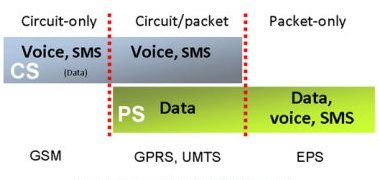
\includegraphics[scale=0.7]{eps.jpg}
  \caption{Domini a circuito e pacchetti}
  \label{fig:eps}
\end{figure}

\subsubsection{Architecture of the EPC}

L'idea dell'architettura EPC è quella di gestire il traffico dati in maniera
 efficiente dal punto di vista delle performance e dei costi

Pochi nodi della rete è coinvolta nella gestione del traffico e le conversioni
 di protocollo vengono evitate.

È stato inoltre deciso di separare i dati degli utenti (\textbf{user plan}) da quelli di segnalazione (noti come \textbf{control plane}) in modo tale rendere
 lo scaling indipendente.
Grazie a questa divisione funzionale, gli operatori possono essere
 dimensionati e adattati alla loro rete facilmente.

\begin{figure}[H]
  \centering
  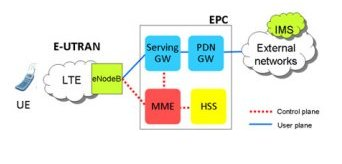
\includegraphics[scale=0.7]{eps_arch.jpg}
  \caption{l'architettura di base degli EPC quando l'UE è connesso all'EPC tramite E-UTRAN(LTE)}
  \label{fig:eps_arch}
\end{figure}

L'Evolved NodeB (eNodeB) è una stazione base per le trasmissioni LTE. Nella
 figura \ref{fig:eps_arch}, l'EPC è composto da 4 elementi di rete:
\begin{itemize}
  \item gateway di servizio (Serving GW);
  \item PDN Gateway (PDN GW);
  \item MME;
  \item HSS.
\end{itemize}

L'EPC è connesso alle reti esterne che possono includere l'IP Multimedia Core 
Network Subsystem (IMS).
